% Slide bảo vệ thực tập: BL Advisor. Biên dịch: xelatex slides.tex (2 lượt).
% Hình riêng: python3 src/make_figures.py; khung ảnh giao diện: python3 src/frame_screenshots.py.
% Quy tắc theo beamer-skill (Noi1r): XeLaTeX, không overlay, tối đa 2 khung màu mỗi slide,
% gạch đầu dòng ngắn, không dùng \tiny, slide tài liệu tham khảo ở vị trí áp chót, slide dự phòng sau \appendix.
% Ghi chú người nói (\note) có thời lượng gợi ý; bật bằng \setbeameroption{show notes on second screen=right}.
\documentclass[aspectratio=169,10pt]{beamer}
\usetheme{Madrid}
\usecolortheme{default}
\setbeamertemplate{navigation symbols}{}
\setbeamertemplate{footline}[frame number]
\setbeamertemplate{bibliography item}[text]

\usepackage{fontspec}
\setmainfont{Liberation Serif}
\setsansfont{Liberation Sans}
\setmonofont{Liberation Mono}

\usepackage{amsmath,amssymb,amsthm,booktabs,mathtools}
\usepackage{stmaryrd}
\usepackage{graphicx}
\usepackage{hyperref}
\usepackage{array}
\usepackage{tikz}
\usetikzlibrary{arrows.meta,positioning,decorations.pathreplacing,calc,shapes.geometric}

% Màu ngữ nghĩa (an toàn cho người khó phân biệt màu). Sắc độ đã tối hơn bản gốc
% để đạt độ tương phản tối thiểu 4,5:1 trên nền trắng (quy tắc 12).
\definecolor{positive}{HTML}{0173B2}
\definecolor{negative}{HTML}{B34700}
\definecolor{emphasis}{HTML}{007A5A}
\definecolor{neutral}{gray}{0.40}
\definecolor{cbPurple}{HTML}{8C3F8B}
\newcommand{\pos}[1]{\textbf{#1}}
\newcommand{\con}[1]{\textcolor{black!50}{#1}}
\newcommand{\HL}[1]{\textbf{#1}}

\renewcommand{\arraystretch}{1.12}
\setlength{\tabcolsep}{5pt}

\newcommand{\fig}[2][0.70]{\includegraphics[width=\linewidth,height=#1\textheight,keepaspectratio]{#2}}
\newcommand{\thumb}[2]{\begin{minipage}[t]{0.235\linewidth}\centering\includegraphics[width=\linewidth,height=2.5cm,keepaspectratio]{img/#1}\\[2pt]#2\end{minipage}}
\let\footnotesize\small
\let\small\normalsize
\newcommand{\src}[1]{{\small\color{neutral}Nguồn: #1}}
\newcommand{\lead}[1]{{\color{structure}\bfseries #1}\par\vspace{5pt}}
\definecolor{accent}{HTML}{008300}
\newcolumntype{L}[1]{>{\raggedright\arraybackslash}p{#1}}

\title[BL Advisor]{BL Advisor: theo dõi danh mục và tối ưu hóa phân bổ tài sản}
\subtitle{Báo cáo thực tập tốt nghiệp}
\author[N. V. Trung]{Nguyễn Văn Trung (K23DTCN418, D23TXCN07K)}
\institute[PTIT]{Học viện Công nghệ Bưu chính Viễn thông\\
Đơn vị thực tập: ITM Semiconductor Vietnam\\
Cán bộ hướng dẫn: ThS. Nguyễn Bá Luận \quad Giảng viên phối hợp: ThS. Vũ Hoài Thư}
\date[29/09/2026]{29/09/2026}
\titlegraphic{
\includegraphics[height=1.8cm]{img/goc/ptit-logo.jpeg}}


\begin{document}

% 1 ------------------------------------------------------------
\begin{frame}
  \titlepage
\end{frame}
\note{0,5 phút. Tổng thời lượng gợi ý: 38 slide chính (trừ slide tham khảo), khoảng 41,5 phút. Bản 30 phút (khoảng 30 phút): giữ slide 1, 3, 4, 9, 7, 8, 10, 17, 18, 19, 20, 21, 22, 23, 25, 26, 27, 30, 32, 33, 34, 35, 36, 39. Bản 20 phút (khoảng 19 phút, còn thời gian hỏi đáp): giữ slide 1, 3, 4, 7, 8, 17, 20, 22, 25, 26, 27, 30, 33, 36, 39. Chào hội đồng, nêu tên đề tài. Cho biết cấu trúc: khái niệm, đơn vị, vấn đề, demo sản phẩm, toán, kết quả.}

% 2 ------------------------------------------------------------
\begin{frame}[t]{Nội dung trình bày}
  \centering\renewcommand{\arraystretch}{1.45}
  \begin{tabular}{@{}rL{4.4cm}L{5.4cm}r@{}}
    \toprule
    & \textbf{Phần} & \textbf{Nội dung} & \textbf{Slide} \\
    \midrule
    1 & Khái niệm và phương pháp & Năm khái niệm, sáu phương pháp & 3 đến 4 \\
    2 & Đơn vị và kế hoạch & Nơi thực tập, 13 tuần & 5 đến 6 \\
    3 & Vấn đề và đóng góp & Vì sao cần công cụ này & 7 đến 9 \\
    4 & Demo sản phẩm & Tám màn hình & 10 đến 16 \\
    5 & Toán và mô hình & Cách máy tính chọn tỷ trọng & 17 đến 28 \\
    6 & Cài đặt & Hệ thống, kiểm tra ngược, giao diện & 29 đến 31 \\
    7 & Kết quả và kết luận & Số liệu, hạn chế, công trình & 32 đến 37 \\
    \bottomrule
  \end{tabular}
\end{frame}
\note{0,5 phút. Nói ngay thông điệp: sản phẩm chạy được; ngoài mẫu, phương pháp Sharpe tối đa lỗ 4,5 phần trăm trong khi chia đều lãi 2,9 phần trăm (dữ liệu demo mô phỏng, một cấu hình). Phần cuối nói rõ.}

% 3 ------------------------------------------------------------
\begin{frame}[t]{Năm khái niệm cần biết trước khi vào phần toán}
  \centering
  \begin{tabular}{@{}L{2.6cm}L{5.6cm}L{4.6cm}@{}}
    \toprule
    \textbf{Khái niệm} & \textbf{Nghĩa đơn giản} & \textbf{Ví dụ} \\
    \midrule
    Lợi suất & Phần trăm lãi hoặc lỗ trong một khoảng thời gian & Đầu tư 100 triệu, được 108 triệu: lợi suất 8\% \\
    Rủi ro (biến động) & Mức giá lên xuống thất thường quanh mức trung bình; càng lớn càng rủi ro & Cổ phiếu lên xuống 5\% mỗi ngày rủi ro hơn quỹ trái phiếu \\
    Tương quan & Hai tài sản có cùng lên, cùng xuống không (từ \(-1\) đến \(1\)) & Hai cổ phiếu ngân hàng thường cùng chiều \\
    Tỷ trọng & Phần trăm vốn đặt vào mỗi tài sản; tổng bằng 100\% & 40 triệu trong 100 triệu: tỷ trọng 40\% \\
    Đa dạng hóa & Chia vốn nhiều nơi để rủi ro chung nhỏ hơn & Cổ phiếu cộng trái phiếu ít cùng giảm \\
    \bottomrule
  \end{tabular}
\end{frame}
\note{1,5 phút. Đọc từng khái niệm bằng ví dụ 100 triệu. Người nghe không cần biết tài chính vẫn theo được phần toán. Nhấn: tương quan thấp là điều kiện để đa dạng hóa có tác dụng.}

% 4 ------------------------------------------------------------
\begin{frame}[t]{Sáu phương pháp phân bổ và hai danh mục chuẩn}
  \centering\small
  \begin{tabular}{@{}L{4.0cm}L{8.6cm}@{}}
    \toprule
    \textbf{Phương pháp} & \textbf{Ý tưởng} \\
    \midrule
    Markowitz, phương sai tối thiểu \cite{markowitz} & Chọn tỷ trọng để rủi ro (biến động) nhỏ nhất \\
    Markowitz, trung bình-phương sai & Cân lợi suất và rủi ro theo mức ngại rủi ro \\
    Markowitz, Sharpe tối đa & Lợi suất vượt lãi phi rủi ro, trên mỗi đơn vị rủi ro, lớn nhất \\
    CVaR tối thiểu & Giảm lỗ trung bình của 5\% ngày tệ nhất (CVaR: giá trị chịu rủi ro có điều kiện) \\
    Cân bằng rủi ro & Mỗi tài sản gây ra phần rủi ro bằng nhau \\
    Black-Litterman & Trộn lợi suất cân bằng của thị trường với quan điểm nhà đầu tư \\
    \midrule
    Hai danh mục chuẩn & Chia đều (1/N) và nghịch đảo biến động (tài sản ít dao động nhận nhiều vốn hơn) \\
    \bottomrule
  \end{tabular}

  Kiểm tra ngược (backtest): chạy lại phương pháp trên quá khứ để xem nó có hiệu quả không.
\end{frame}
\note{1,5 phút. Bảng tra nhanh sáu phương pháp; quay lại khi gặp tên phương pháp ở phần sau. Markowitz có ba biến thể. Kiểm tra ngược là chạy lại trên quá khứ.}

% 5 ------------------------------------------------------------
\begin{frame}[t]{Đơn vị thực tập: ITM Semiconductor Vietnam (ITMV)}
  \centering
  \begin{tabular}{@{}L{3.6cm}L{9.6cm}@{}}
    \toprule
    \textbf{Nội dung} & \textbf{Thông tin} \\
    \midrule
    Loại hình & Công ty TNHH một thành viên, 100\% vốn Hàn Quốc, thuộc tập đoàn ITM \\
    Địa điểm & Khu công nghiệp VSIP Bắc Ninh; ba nhà máy V1, V2, V3 \\
    Sản phẩm & Vi mạch bảo vệ một chip (POC), mô-đun bảo vệ pin (PMP), bộ pin, ăng-ten NFC (giao tiếp trường gần) \\
    Quy mô & Khoảng 3.500 lao động (năm 2024) \\
    Thời gian & 13 tuần, 01/07/2026 đến 27/09/2026 \\
    Vị trí sinh viên & Dự án học tập độc lập, báo cáo tiến độ hằng tuần cho cán bộ hướng dẫn \\
    \bottomrule
  \end{tabular}
\end{frame}
\note{1 phút. NFC là giao tiếp trường gần. Dự án không thuộc phòng ban nào của công ty; số 3.500 lao động là số công khai, chưa đối chiếu nội bộ. Sơ đồ tổ chức ở slide dự phòng 1.}

% 6 ------------------------------------------------------------
\begin{frame}[t]{Kế hoạch thực tập: 13 tuần, năm giai đoạn}
  \centering
  \begin{tikzpicture}[x=0.72cm, y=0.66cm, every node/.style={font=\small}]
    \foreach \w in {1,...,13}{
      \node[font=\footnotesize, text=neutral] at (\w-0.5,0.6) {\w};
      \draw[black!12] (\w-1,0.2) -- (\w-1,-5.3);
    }
    \draw[black!12] (13,0.2) -- (13,-5.3);
    \node[font=\footnotesize, text=neutral, anchor=east] at (0,0.6) {Tuần};
    \foreach \i/\a/\b/\t in {
      1/1/2/{Khởi động, chọn đề tài},
      2/3/4/{Lý thuyết và Việt hóa},
      3/5/8/{Thuật toán, dữ liệu, API},
      4/9/10/{Giao diện tối ưu hóa},
      5/11/13/{Kiểm thử và hoàn thiện}}{
      \node[anchor=east, align=right] at (-0.15,-\i+0.3) {\t};
      \draw[accent, fill=accent!65, rounded corners=2pt] (\a-1+0.06,-\i+0.65) rectangle (\b-0.06,-\i-0.05);
    }
    \foreach \x/\i in {1/1, 8/3, 9/4, 11/5, 13/5}{
      \node[diamond, fill=black, inner sep=1.8pt] at (\x,-\i+0.3) {};
    }
  \end{tikzpicture}

  {\small Mốc (hình thoi): tuần 1 chốt đề tài; tuần 8 điểm cuối tối ưu hóa (API: giao diện để các phần mềm gọi nhau); tuần 9 trang tối ưu hóa; tuần 11 kiểm thử độc lập vòng 1; tuần 13 đóng gói và báo cáo.}

  \vspace{2pt}
\end{frame}
\note{1 phút. Năm giai đoạn là cách nhóm của sinh viên. API là giao diện lập trình ứng dụng; điểm cuối là địa chỉ máy chủ nhận yêu cầu. Kiểm thử độc lập vòng 1 ở tuần 11.}

% 7 ------------------------------------------------------------
\begin{frame}[t]{Vấn đề: nhà đầu tư cá nhân Việt Nam thiếu công cụ phù hợp}
  \begin{columns}[T]
    \begin{column}{0.56\textwidth}
      \begin{tabular}{@{}L{2.5cm}L{4.4cm}@{}}
        \toprule
        \textbf{Cách đang dùng} & \textbf{Hạn chế} \\
        \midrule
        Bảng tính & Dễ sai công thức; không tự cập nhật giá; không đo rủi ro \\
        Phần mềm nước ngoài & Không có tiếng Việt; mặc định USD; số theo quy ước Anh Mỹ \\
        Mã nguồn mở có sẵn & Chỉ theo dõi và trình bày; ít khi gợi ý phân bổ \\
        \bottomrule
      \end{tabular}
    \end{column}
    \begin{column}{0.42\textwidth}
      \centering
      \begin{tikzpicture}[every node/.style={font=\normalsize}, box/.style={draw, rounded corners, align=center, minimum width=3.8cm, minimum height=0.9cm}]
        \node[box, draw=accent] (in) at (0,2.0) {Người dùng gõ \textbf{1.000}};
        \node[box, draw=accent] (vn) at (0,0.5) {Việt Nam: \textbf{một nghìn}};
        \node[box, draw=negative] (us) at (0,-1.0) {Anh Mỹ: \textbf{một} (1,0)};
        \draw[-{Stealth[length=2.5mm]}, thick] (in) -- (vn);
        \draw[-{Stealth[length=2.5mm]}, thick] (vn) -- (us);
      \end{tikzpicture}

      Nhầm dấu chấm và dấu phẩy khi nhập tiền
    \end{column}
  \end{columns}
\end{frame}
\note{1 phút. Khoảng trống của đề tài: công cụ tiếng Việt, tiền VND, có gợi ý phân bổ. Ví dụ 1.000: người Việt đọc một nghìn, phần mềm Anh Mỹ đọc một.}

% 8 ------------------------------------------------------------
\begin{frame}[t]{Ba câu hỏi nghiên cứu và ba giả thuyết kiểm chứng}
  \begin{columns}[T]
    \begin{column}{0.48\textwidth}
      \begin{tabular}{@{}L{1.0cm}L{4.9cm}@{}}
        \toprule
        \textbf{Câu} & \textbf{Câu hỏi nghiên cứu} \\
        \midrule
        CH1 & Mở rộng nền tảng mã nguồn mở thành bản tiếng Việt, tiền VND, không viết lại? \\
        CH2 & Sáu phương pháp phân bổ trong một máy chủ TypeScript, tối đa 20 tài sản, dưới 5 giây? \\
        CH3 & Kiểm chứng thuật toán bằng kiểm thử theo tính chất toán học? \\
        \bottomrule
      \end{tabular}
    \end{column}
    \begin{column}{0.48\textwidth}
      \begin{tabular}{@{}L{1.6cm}L{4.4cm}@{}}
        \toprule
        \textbf{Giả thuyết} & \textbf{Nội dung} \\
        \midrule
        H1 & Tối ưu hóa kèm kiểm tra ngược chạy dưới 5 giây trên dữ liệu demo \\
        H2 & Tỷ trọng không âm, cộng bằng 1, không vượt trần (trừ cân bằng rủi ro) \\
        H3 & Quan điểm tăng giá, tin cậy cao, làm tăng tỷ trọng tài sản đó \\
        \bottomrule
      \end{tabular}
    \end{column}
  \end{columns}
\end{frame}
\note{1 phút. Nhấn: cân bằng rủi ro chưa áp trần tỷ trọng, nên H2 loại trừ phương pháp này.}

% 9 ------------------------------------------------------------
\begin{frame}[t]{Đóng góp của sinh viên trên nền Ghostfolio}
  \centering
  \begin{tabular}{@{}L{5.2cm}L{7.6cm}@{}}
    \toprule
    \textbf{Đóng góp} & \textbf{Kết quả} \\
    \midrule
    Việt hóa, định dạng số vi-VN & Ô nhập tự thêm dấu chấm ngăn cách khi gõ \\
    Mô-đun tối ưu hóa bằng TypeScript thuần & Sáu phương pháp, đường biên hiệu quả \\
    Black-Litterman có quan điểm & Tuyệt đối và tương đối, tin cậy 5\% đến 95\% \\
    Kiểm tra ngược walk-forward & Chỉ dùng dữ liệu trước mỗi kỳ cân bằng lại \\
    Bộ dữ liệu demo tái lập được & 16 tài khoản, 4.519 giao dịch, 22 tài sản, 4 chỉ số \\
    Kiểm thử & Ít nhất 44 bài do sinh viên viết (37 tối ưu hóa, 7 nhập số) \\
    \bottomrule
  \end{tabular}

  \vspace{6pt}
  Phần còn lại (theo dõi danh mục, FIRE, X-ray) là của Ghostfolio, giấy phép AGPL-3.0 \cite{agpl}.
\end{frame}
\note{1 phút. Phần lớn chức năng quản lý danh mục là của Ghostfolio. Đóng góp riêng gồm sáu điểm trong bảng; 501 bài kiểm thử là của cả kho, riêng phần sinh viên viết ít nhất 44 bài.}

% 10 ------------------------------------------------------------
\begin{frame}[t]{Demo sản phẩm: tám màn hình của BL Advisor}
  \centering
  \thumb{fr-full-tong-quan.png}{1. Tổng quan}\hfill
  \thumb{fr-full-giao-dich.png}{2. Giao dịch}\hfill
  \thumb{fr-full-phan-tich.png}{3. Phân tích}\hfill
  \thumb{fr-full-fire.png}{4. FIRE}

  \vspace{8pt}
  \thumb{fr-full-xray.png}{5. X-ray}\hfill
  \thumb{fr-full-thi-truong.png}{6. Thị trường}\hfill
  \thumb{fr-quan-tri.png}{7. Quản trị}\hfill
  \thumb{fr-di-dong.png}{8. Điện thoại}

  \vspace{8pt}
  Tiếng Việt, tiền VND, số theo quy ước Việt Nam
\end{frame}
\note{0,5 phút. Điểm qua tám màn hình sắp xem: tổng quan, giao dịch, phân tích, FIRE, X-ray, thị trường, quản trị, điện thoại.}

% 11 ------------------------------------------------------------
\begin{frame}[t]{Sản phẩm 1: một trang cho toàn bộ danh mục, tính bằng VND}
  \begin{columns}[T]
    \begin{column}{0.60\textwidth}
      \centering\fig[0.70]{img/fr-full-tong-quan.png}
    \end{column}
    \begin{column}{0.37\textwidth}
      \begin{itemize}
        \item Con số lớn: tài sản ròng, bằng VND
        \item Đường: diễn biến tài sản theo thời gian
        \item Menu trái: Tổng quan, Khoản nắm giữ, Thị trường
      \end{itemize}
    \end{column}
  \end{columns}

\end{frame}
\note{0,5 phút. Tài sản ròng bằng VND, gom mọi loại tài sản. Chức năng nền của Ghostfolio, sinh viên đổi sang VND và tiếng Việt.}

% 12 ------------------------------------------------------------
\begin{frame}[t]{Sản phẩm 2: nhập số theo cách người Việt viết}
  \begin{columns}[T]
    \begin{column}{0.52\textwidth}
      \centering
      \begin{tikzpicture}[every node/.style={font=\Large}, field/.style={draw, rounded corners, minimum width=5.2cm, minimum height=1.1cm, align=left, inner xsep=8pt}]
        \node[font=\normalsize, anchor=west] at (0,1.9) {Số lượng};
        \node[field, draw=structure, very thick, anchor=west] at (0,1.2) {\textbf{1.234.567}};
        \node[font=\normalsize, anchor=west] at (0,0.1) {Đơn giá};
        \node[field, draw=structure, very thick, anchor=west] at (0,-0.6) {\textbf{85.000,5}};
      \end{tikzpicture}

      Gõ \textbf{1234567}, ô tự thêm dấu chấm
    \end{column}
    \begin{column}{0.45\textwidth}
      \centering\fig[0.62]{img/fr-full-giao-dich.png}
    \end{column}
  \end{columns}

  \vspace{4pt}
  \begin{itemize}\raggedright
    \item Dấu chấm ngăn hàng nghìn, dấu phẩy là phần thập phân
    \item Một thành phần dùng lại (directive) cho mọi ô số; 7 bài kiểm thử
  \end{itemize}
\end{frame}
\note{0,5 phút. Phần Việt hóa cụ thể nhất; ví dụ 1.000 ở slide vấn đề quay lại ở đây. Ô nhập tự thêm dấu chấm khi gõ.}

% 13 ------------------------------------------------------------
\begin{frame}[t]{Sản phẩm 3: trang Phân tích cho biết hiệu suất và so sánh chỉ số}
  \begin{columns}[T]
    \begin{column}{0.60\textwidth}
      \centering\fig[0.70]{img/fr-full-phan-tich.png}
    \end{column}
    \begin{column}{0.37\textwidth}
      \begin{itemize}
        \item Ba ô: tổng số tiền, thay đổi, hiệu suất
        \item Hai đường: danh mục và VN-Index mô phỏng
        \item Thay đổi có tính đến ảnh hưởng của tỷ giá
      \end{itemize}
    \end{column}
  \end{columns}

\end{frame}
\note{0,5 phút. Ba ô số ở trên là tổng số tiền, thay đổi và hiệu suất; đường biểu diễn so danh mục với VN-Index mô phỏng.}

% 14 ------------------------------------------------------------
\begin{frame}[t]{Sản phẩm 4 và 5: công cụ FIRE và kiểm tra rủi ro X-ray}
  \begin{columns}[T]
    \begin{column}{0.49\textwidth}
      \centering\fig[0.55]{img/fr-full-fire.png}

      FIRE (nghỉ hưu sớm): rút bền vững 74.100.295,91 VND mỗi năm, tỷ lệ 4,0\%
    \end{column}
    \begin{column}{0.49\textwidth}
      \centering\fig[0.55]{img/fr-full-xray.png}

      X-ray: 2 trên tổng 16 quy tắc rủi ro phù hợp với danh mục demo
    \end{column}
  \end{columns}

  \vspace{4pt}
  Hai chức năng có sẵn từ Ghostfolio; sinh viên Việt hóa số nhập và tiền tệ
\end{frame}
\note{0,5 phút. FIRE là độc lập tài chính, nghỉ hưu sớm; X-ray kiểm tra 16 quy tắc rủi ro. Hai chức năng có sẵn từ Ghostfolio, sinh viên Việt hóa số nhập.}

% 15 ------------------------------------------------------------
\begin{frame}[t]{Sản phẩm 6 và 7: trang Thị trường và trang Quản trị}
  \begin{columns}[T]
    \begin{column}{0.49\textwidth}
      \centering\fig[0.50]{img/fr-full-thi-truong.png}

      Bốn chỉ số mô phỏng: Bitcoin, S\&P 500, VN-Index, VN30
    \end{column}
    \begin{column}{0.49\textwidth}
      \centering\fig[0.50]{img/fr-quan-tri.png}

      Quản trị: 16 người dùng, 4.519 giao dịch (282,44 mỗi người)
    \end{column}
  \end{columns}

  \vspace{4pt}
  Quản trị viên bật tắt đăng ký người dùng, thu thập dữ liệu và xóa bộ nhớ đệm
\end{frame}
\note{0,5 phút. Trang Thị trường theo dõi bốn chỉ số mô phỏng; trang Quản trị cho quản trị viên: số người dùng, giao dịch, bật tắt đăng ký, xóa bộ nhớ đệm.}

% 16 ------------------------------------------------------------
\begin{frame}[t]{Sản phẩm 8: giao diện thích ứng trên điện thoại}
  \begin{columns}[T]
    \begin{column}{0.40\textwidth}
      \centering\fig[0.76]{img/fr-di-dong.png}
    \end{column}
    \begin{column}{0.57\textwidth}
      \begin{itemize}
        \item Cùng hệ thống, hiển thị theo màn hình điện thoại
        \item Giá trị khoản nắm giữ, biểu đồ giá, danh sách giao dịch
      \end{itemize}
    \end{column}
  \end{columns}

\end{frame}
\note{0,5 phút. Cùng hệ thống hiển thị trên điện thoại; ví dụ khoản FPT Corp với biểu đồ giá và danh sách giao dịch.}

% 17 ------------------------------------------------------------
\begin{frame}[t]{Toán 1: từ chuỗi giá đến hai đại lượng cho mô hình}
  \lead{Trước khi tính, máy cần biết gì về mỗi tài sản?}
  \begin{columns}[T]
    \begin{column}{0.48\textwidth}
      \begin{itemize}
        \item Cần lợi suất kỳ vọng \(\mu\) và mức cùng lên xuống \(\Sigma\); quy từ ngày ra năm bằng 252
      \end{itemize}
      \[ \mu_i = 252\,\bar r_i, \qquad \Sigma = 252\,\operatorname{Cov}(r) \]
      {\small \(\bar r_i\): lợi suất ngày trung bình; \(\Sigma\): ma trận hiệp phương sai.}

      \vspace{3pt}
      {\small Ví dụ: NVIDIA \(0{,}118\%\times 252\approx 29{,}7\%\) mỗi năm.}
    \end{column}
    \begin{column}{0.48\textwidth}
      \small\setlength{\tabcolsep}{3pt}
      \begin{tabular}{@{}lrr@{}}
        \toprule
        Tài sản & Lợi suất \(\mu_i\) & Biến động \(\sigma_i\) \\
        \midrule
        NVIDIA & 29,7\% & 56,2\% \\
        FPT & 12,1\% & 32,5\% \\
        Vietcombank & 10,2\% & 27,3\% \\
        Vinamilk & 9,9\% & 26,8\% \\
        Quỹ trái phiếu & 9,5\% & 2,9\% \\
        Vanguard S\&P 500 & 8,6\% & 17,0\% \\
        Hòa Phát & \con{−4,1\%} & 40,1\% \\
        Microsoft & \con{−3,8\%} & 25,9\% \\
        \bottomrule
      \end{tabular}

    \end{column}
  \end{columns}
\end{frame}
\note{1,5 phút. Ví dụ: NVIDIA 0,118 phần trăm mỗi ngày nhân 252 được 29,7 phần trăm mỗi năm. Hệ số 252 gây thấp lợi suất khi có tiền mã hóa (hạn chế đã ghi trong báo cáo).}

% 18 ------------------------------------------------------------
\begin{frame}[t]{Toán 2: tương quan cho thấy vì sao đa dạng hóa có tác dụng}
  \lead{Vì sao chia vốn nhiều nơi giảm rủi ro? Nhìn tương quan giữa ba nhóm tài sản.}
  \begin{columns}[T]
    \begin{column}{0.55\textwidth}
      \centering\fig[0.70]{img/hinh-tuong-quan.png}
    \end{column}
    \begin{column}{0.42\textwidth}
      \begin{itemize}
        \item Cùng nhóm: tương quan trung bình 0,38
        \item Khác nhóm: 0,04
        \item Tương quan thấp: hai tài sản ít cùng giảm, nên rủi ro chung nhỏ hơn
        \item Nhóm: cổ phiếu Việt Nam, tài sản Mỹ, quỹ trái phiếu; dữ liệu mô phỏng
      \end{itemize}
    \end{column}
  \end{columns}
\end{frame}
\note{1,5 phút. Đọc hình: cột xanh là tương quan trung bình cùng nhóm, 0,38; cột xám là khác nhóm, 0,04. Trung thực: dữ liệu mô phỏng làm tương quan giữa các nhóm thấp hơn thực tế.}

% 19 ------------------------------------------------------------
\begin{frame}[t]{Toán 3: hai tài sản, rủi ro chung giảm khi tương quan thấp}
  \lead{Tương quan thấp giúp được bao nhiêu? Thử với Vinamilk và Vietcombank, mỗi cổ phiếu biến động khoảng 27\%.}
  \begin{columns}[T]
    \begin{column}{0.53\textwidth}
      \centering\fig[0.66]{img/hinh-da-dang-hoa.png}
    \end{column}
    \begin{column}{0.44\textwidth}
      \[ \sigma_p^2=w^2\sigma_1^2+(1-w)^2\sigma_2^2+2w(1-w)\rho\,\sigma_1\sigma_2 \]
      {\small \(w\): tỷ trọng tài sản 1; \(\rho\): tương quan; \(\sigma_p\): biến động danh mục.}

      \vspace{4pt}
      Ví dụ: \(\rho=0{,}38\), hai biến động 26,8\% và 27,3\%, chia đôi: còn 22,5\%.
    \end{column}
  \end{columns}
\end{frame}
\note{1,5 phút. Ví dụ tính tay: w bằng 0,5, hai biến động khoảng 27 phần trăm, tương quan 0,38, ra 22,5 phần trăm. Tương quan càng thấp, đường càng lõm sâu.}

% 20 ------------------------------------------------------------
\begin{frame}[t]{Toán 4: Markowitz đặt bài toán tối ưu}
  \lead{Đã biết đa dạng hóa giảm rủi ro. Vậy chia vốn thế nào là tốt nhất?}
  \begin{columns}[T]
    \begin{column}{0.48\textwidth}
      \begin{itemize}
        \item Lợi suất trừ phần phạt rủi ro càng lớn càng tốt \cite{markowitz}
        \item \(\delta\): mức ngại rủi ro; \(c\): trần tỷ trọng, ở đây 40\%
      \end{itemize}
      \[ \max_{w}\ \mu^{\top}w-\tfrac{\delta}{2}\,w^{\top}\Sigma\,w \]
      \[ \textstyle\sum_i w_i=1,\qquad 0\le w_i\le c \]
    \end{column}
    \begin{column}{0.48\textwidth}
      \textbf{Ví dụ: hai tài sản, \(\delta=4\)}

      {\small A: \(\mu=12\%\), \(\sigma=30\%\); B: \(\mu=6\%\), \(\sigma=10\%\); không tương quan.}
      \vspace{2pt}

      \begin{tabular}{@{}rrrr@{}}
        \toprule
        \(w_A\) & \(\mu_p\) & \(\sigma_p^2\) & Điểm \\
        \midrule
        0\% & 6,0\% & 0,0100 & 0,0400 \\
        25\% & 7,5\% & 0,0113 & \textbf{0,0525} \\
        50\% & 9,0\% & 0,0250 & 0,0400 \\
        100\% & 12,0\% & 0,0900 & \(-0{,}0600\) \\
        \bottomrule
      \end{tabular}

      \vspace{2pt}
      {\small Điểm \(=\mu_p-2\sigma_p^2\); tốt nhất tại \(w_A=25\%\).}
    \end{column}
  \end{columns}
\end{frame}
\note{1,5 phút. Đọc ví dụ hai tài sản: thử bốn tỷ trọng, điểm cao nhất ở 25 phần trăm tài sản A. Đó chính là việc máy tính làm, nhưng cho tám tài sản.}

% 21 ------------------------------------------------------------
\begin{frame}[t]{Toán 5: đường biên hiệu quả}
  \lead{Mỗi mức ngại rủi ro \(\delta\) cho một nghiệm khác nhau. Các nghiệm nằm ở đâu?}
  \begin{columns}[T]
    \begin{column}{0.56\textwidth}
      \centering\fig[0.66]{img/hinh-duong-bien.png}
    \end{column}
    \begin{column}{0.41\textwidth}
      \begin{itemize}
        \item Mỗi điểm trên đường: lợi suất cao nhất ở một mức rủi ro
        \item Hiện tại nằm dưới đường: cùng rủi ro, lãi thấp hơn
        \item Sharpe tối đa (xem slide sau): lãi 11,2\% (hiện tại 11,9\%), biến động 10,0\% (18,1\%)
      \end{itemize}
    \end{column}
  \end{columns}
\end{frame}
\note{1,5 phút. Trong mẫu: Sharpe tối đa có lợi suất 11,2 phần trăm so với 11,9, mà biến động chỉ 10 thay vì 18,1. Hình chỉ vẽ ba danh mục; bảng đủ ở phần kết quả trong mẫu.}

% 22 ------------------------------------------------------------
\begin{frame}[t]{Toán 6: Sharpe tối đa}
  \lead{Trên đường biên có vô số điểm. Chọn điểm nào?}
  \begin{columns}[T]
    \begin{column}{0.48\textwidth}
      \begin{itemize}
        \item Lãi vượt lãi phi rủi ro, chia cho rủi ro, càng cao càng tốt \cite{sharpe}
        \item Nếu nghiệm vượt trần 40\%, đưa về điểm hợp lệ gần nhất
      \end{itemize}
      \[ S(w)=\frac{\mu^{\top}w-r_f}{\sqrt{w^{\top}\Sigma\,w}} \]
      {\small \(r_f\): lãi suất phi rủi ro, ở đây 3\%/năm.}
    \end{column}
    \begin{column}{0.48\textwidth}
      \textbf{Ví dụ: tám tài sản, trần 40\%}
      \vspace{2pt}

      \setlength{\tabcolsep}{3pt}
      \begin{tabular}{@{}lrr@{}}
        \toprule
        Tài sản & Hiện tại & Sharpe tối đa \\
        \midrule
        Quỹ trái phiếu & 13,4\% & \pos{40,0\%} \\
        Vanguard S\&P 500 & 12,1\% & \pos{27,0\%} \\
        NVIDIA & 22,0\% & 7,7\% \\
        Hòa Phát & 8,8\% & \con{0,0\%} \\
        Microsoft & 8,4\% & \con{0,0\%} \\
        \bottomrule
      \end{tabular}

      \vspace{2pt}
      {\small Trần 40\% chặn quỹ trái phiếu.}
    \end{column}
  \end{columns}
\end{frame}
\note{1,5 phút. Quỹ trái phiếu ít biến động nên được dồn tới đúng trần 40 phần trăm. Hai tài sản lợi suất âm bị đưa về 0.}

% 23 ------------------------------------------------------------
\begin{frame}[t]{Toán 7: CVaR nhìn vào những ngày tệ nhất}
  \lead{Phương sai coi lãi và lỗ như nhau. Có thước đo nào chỉ nhìn phần lỗ?}
  \begin{columns}[T]
    \begin{column}{0.50\textwidth}
      \centering\fig[0.66]{img/hinh-cvar.png}
    \end{column}
    \begin{column}{0.47\textwidth}
      \begin{itemize}
        \item Vùng xanh lá: 5\% ngày tệ nhất; CVaR là lỗ trung bình của vùng đó \cite{rockafellar}
      \end{itemize}
      \[ \mathrm{CVaR}_{\alpha}(w)=\frac{1}{k}\sum_{j=1}^{k}\ell_{(j)}(w) \]
      {\small \(\alpha\): mức tin cậy (95\%); \(T\): số ngày; \(\ell_{(j)}\): mức lỗ lớn thứ \(j\); \(k=\lceil(1-\alpha)T\rceil\).}

      \vspace{2pt}
      Ví dụ (dữ liệu demo mô phỏng): \(T=521\), \(k=27\) ngày tệ nhất, lỗ trung bình 2,15\% một ngày; CVaR tối thiểu chỉ còn 1,03\%.
    \end{column}
  \end{columns}
\end{frame}
\note{1,5 phút. Vùng xanh lá trên hình là 5 phần trăm ngày tệ nhất, 27 ngày. Trung bình lỗ của các ngày đó là 2,15 phần trăm.}

% 24 ------------------------------------------------------------
\begin{frame}[t]{Toán 8: cân bằng rủi ro, mỗi tài sản gánh phần như nhau}
  \lead{Cách khác, không cần đoán lợi suất: chia rủi ro đều thay vì chia vốn đều.}
  \begin{columns}[T]
    \begin{column}{0.53\textwidth}
      \centering\fig[0.66]{img/hinh-dong-gop-rui-ro.png}
    \end{column}
    \begin{column}{0.44\textwidth}
      \begin{itemize}
        \item Chỉ cần hiệp phương sai, không cần lợi suất kỳ vọng \cite{maillard}
        \item NVIDIA: 22\% vốn nhưng 55,6\% rủi ro
        \item Quỹ trái phiếu (biến động 2,9\%) nhận 65\% vốn; Sharpe tối đa bị chặn ở 40\%
      \end{itemize}
      \[ w_i(\Sigma w)_i = w_j(\Sigma w)_j \quad \forall\, i,j \]
      {\small \(w_i(\Sigma w)_i\): phần rủi ro do tài sản \(i\) gánh. Dữ liệu demo mô phỏng.}
    \end{column}
  \end{columns}
\end{frame}
\note{1,5 phút. Điểm dễ hiểu nhất: NVIDIA chiếm 22 phần trăm tỷ trọng nhưng 55,6 phần trăm phương sai. Đừng nhầm với biến động riêng 56,2 phần trăm.}

% 25 ------------------------------------------------------------
\begin{frame}[t]{Toán 9: Black-Litterman, thêm quan điểm của bạn}
  \lead{Lợi suất lịch sử nhiễu. Black-Litterman xuất phát từ lợi suất cân bằng của thị trường, rồi điều chỉnh theo quan điểm.}
  \begin{columns}[T]
    \begin{column}{0.50\textwidth}
      \begin{itemize}
        \item Prior \(\pi\): lợi suất mà thị trường ngầm định, không dùng lịch sử \cite{blitterman,heLitterman}
        \item Trộn với quan điểm nhà đầu tư, ra hậu nghiệm (ước lượng sau khi thêm quan điểm)
      \end{itemize}
      \[ \pi=\delta\,\Sigma\,w_{\mathrm{mkt}} \]
      {\small \(\pi\): lợi suất cân bằng; \(w_{\mathrm{mkt}}\): ở ứng dụng là danh mục hiện tại.}
    \end{column}
    \begin{column}{0.45\textwidth}
      \centering
      \begin{tikzpicture}[node distance=0.55cm, every node/.style={font=\normalsize},
        box/.style={draw, rounded corners, align=center, text width=4.8cm, minimum height=0.8cm},
        arr/.style={-{Stealth[length=2.5mm]}, thick}]
        \node[box] (a) {Lợi suất cân bằng \(\pi\)};
        \node[box, below=of a] (b) {Quan điểm và độ tin cậy};
        \node[box, below=of b] (c) {Lợi suất hậu nghiệm};
        \node[box, below=of c] (d) {Tối ưu hóa không âm, có trần};
        \draw[arr] (a) -- (b);
        \draw[arr] (b) -- (c);
        \draw[arr] (c) -- (d);
      \end{tikzpicture}
    \end{column}
  \end{columns}
\end{frame}
\note{1,5 phút. Ý tưởng: bắt đầu từ lợi suất cân bằng, rồi chỉnh theo quan điểm. Nói rõ quy ước: danh mục hiện tại đóng vai tỷ trọng thị trường.}

% 26 ------------------------------------------------------------
\begin{frame}[t]{Toán 10: độ tin cậy quyết định quan điểm nặng bao nhiêu}
  \lead{Mỗi quan điểm nặng bao nhiêu trong kết quả? Tùy độ tin cậy.}
  \begin{columns}[T]
    \begin{column}{0.48\textwidth}
      \begin{itemize}
        \item Tin cậy 5\% đến 95\%: càng cao, quan điểm càng nặng (Idzorek \cite{idzorek})
      \end{itemize}
      \[ \Omega_{kk}=\tau\,p_k^{\top}\Sigma\,p_k\,\frac{1-c_k}{c_k} \]
      {\small \(\Omega_{kk}\): độ bất định của quan điểm \(k\); \(c_k\): độ tin cậy; \(\tau\): độ bất định của prior.}
    \end{column}
    \begin{column}{0.48\textwidth}
      \textbf{Ví dụ: hệ số \((1-c)/c\)}
      \vspace{2pt}

      \begin{tabular}{@{}rrL{3.3cm}@{}}
        \toprule
        \textbf{Tin cậy} & \textbf{Hệ số} & \textbf{Ý nghĩa} \\
        \midrule
        5\% & 19 & Gần như bỏ qua \\
        50\% & 1 & Nặng bằng prior \\
        60\% & 0,67 & Quan điểm Vinamilk \\
        95\% & 0,05 & Gần như tin hoàn toàn \\
        \bottomrule
      \end{tabular}
    \end{column}
  \end{columns}
\end{frame}
\note{1 phút. Bảng hệ số (1 trừ c) chia c: tin cậy 95 phần trăm gần như tin hoàn toàn, 5 phần trăm gần như bỏ qua.}

% 27 ------------------------------------------------------------
\begin{frame}[t]{Toán 11: lợi suất hậu nghiệm dịch về phía quan điểm}
  \lead{Hậu nghiệm là trung bình có trọng số của prior và các quan điểm; quan điểm tin cậy hơn thì nặng hơn. Kết quả ra sao?}
  \begin{columns}[T]
    \begin{column}{0.48\textwidth}
      \centering\fig[0.62]{img/hinh-bl-hau-nghiem.png}
    \end{column}
    \begin{column}{0.49\textwidth}
      \[ \begin{aligned} M&=(\tau\Sigma)^{-1}+P^{\top}\Omega^{-1}P\\ E[R]&=M^{-1}\bigl[(\tau\Sigma)^{-1}\pi+P^{\top}\Omega^{-1}Q\bigr] \end{aligned} \]
      {\small \(P,Q\): quan điểm và lợi suất chúng nêu; \(M\): độ chính xác gộp; \(\tau\): độ bất định của prior. Dữ liệu demo mô phỏng; \(\delta=2{,}5\), \(\tau=5\%\).}
      \begin{itemize}
        \item Quan điểm 1: Vinamilk 12\%, tin cậy 60\%; quan điểm 2: FPT vượt Vietcombank 3\%, tin cậy 50\%
        \item Vinamilk 5,5\% lên 9,4\%; FPT 5,8\% lên 8,6\%
        \item Vietcombank 6,4\% lên 7,3\% (riêng quan điểm 1: 7,9\%; riêng quan điểm 2: 5,7\%)
      \end{itemize}
    \end{column}
  \end{columns}
\end{frame}
\note{1,5 phút. Quan điểm 2 là tương đối: FPT vượt Vietcombank 3 phần trăm mỗi năm, tin cậy 50. Vietcombank vẫn tăng vì tương quan 0,38 với Vinamilk. Sau bước này ứng dụng giải bài toán trung bình-phương sai có trần trên lợi suất hậu nghiệm.}

% 28 ------------------------------------------------------------
\begin{frame}[t]{Black-Litterman trên giao diện: nhập hai quan điểm}
  \begin{columns}[T]
    \begin{column}{0.60\textwidth}
      \centering\fig[0.70]{img/fr-full-bl.png}
    \end{column}
    \begin{column}{0.37\textwidth}
      \begin{itemize}
        \item Nhập trực tiếp hai quan điểm, mỗi quan điểm một độ tin cậy
        \item Ảnh chụp đặt trần 35\%; các slide toán dùng 40\%
        \item Kiểm thử: tin cậy 90\% làm tăng tỷ trọng và lợi suất hậu nghiệm
      \end{itemize}
    \end{column}
  \end{columns}

\end{frame}
\note{1 phút. Hai quan điểm nhập trực tiếp trên giao diện; hộp chọn tài sản đang mở.}

% 29 ------------------------------------------------------------
\begin{frame}[t]{Cài đặt 1: kiến trúc và luồng xử lý một yêu cầu tối ưu hóa}
  \centering
  \begin{tikzpicture}[every node/.style={font=\normalsize, align=center}, box/.style={draw, rounded corners, minimum height=1.1cm, minimum width=3.0cm, thick},
    arr/.style={-{Stealth[length=2.5mm]}, very thick}]
    \node[box] (web) at (0,0) {Trình duyệt\\(Angular)};
    \node[box, draw=structure, fill=structure!12] (api) at (4.6,0) {Máy chủ API (NestJS)\\mô-đun tối ưu hóa};
    \node[box] (db) at (9.4,0.9) {PostgreSQL: dữ liệu};
    \node[box] (redis) at (9.4,-0.4) {Redis: bộ nhớ đệm};
    \node[box] (ext) at (9.4,-1.7) {Nguồn giá ngoài};
    \draw[arr] (web) -- (api);
    \draw[arr] (api) -- (db); \draw[arr] (api) -- (redis); \draw[arr] (api) -- (ext);
  \end{tikzpicture}

  \vspace{10pt}
  \begin{tikzpicture}[every node/.style={font=\normalsize, align=center}, box/.style={draw, rounded corners, minimum height=1.0cm, minimum width=1.9cm, thick},
    arr/.style={-{Stealth[length=2.5mm]}, very thick}]
    \node[box] (a) at (0,0) {1. Nhận\\yêu cầu};
    \node[box] (b) at (2.3,0) {2. Lấy giá,\\khoản giữ};
    \node[box] (c) at (4.6,0) {3. Căn giá,\\đổi VND};
    \node[box] (d) at (6.9,0) {4. Ước\\lượng};
    \node[box, draw=structure, fill=structure!12] (e) at (9.2,0) {5. Chạy\\phương pháp};
    \node[box] (f) at (11.5,0) {6. Kiểm tra\\ngược};
    \foreach \x/\y in {a/b,b/c,c/d,d/e,e/f}{\draw[arr] (\x) -- (\y);}
  \end{tikzpicture}

  \vspace{6pt}
  Căn giá không nhìn trước dữ liệu tương lai; tối đa 20 tài sản mỗi yêu cầu
\end{frame}
\note{1,5 phút. Hàng trên: trình duyệt gọi API NestJS, dữ liệu ở PostgreSQL, bộ nhớ đệm Redis. Hàng dưới: sáu bước của một yêu cầu; căn giá không nhìn trước dữ liệu tương lai.}

% 30 ------------------------------------------------------------
\begin{frame}[t]{Cài đặt 2: kiểm tra ngược (backtest) walk-forward}
  \begin{columns}[T]
    \begin{column}{0.44\textwidth}
      \begin{itemize}
        \item Ước lượng từ 252 ngày gần nhất, giữ danh mục 63 ngày rồi cân bằng lại
        \item Trong mẫu: dùng cả dữ liệu để chọn và đo; ngoài mẫu: đo trên phần chưa thấy
        \item Chưa tính phí, thuế, trượt giá
      \end{itemize}
    \end{column}
    \begin{column}{0.53\textwidth}
      \centering
      \begin{tikzpicture}[x=1.22cm, y=1.2cm, every node/.style={font=\normalsize}]
        \draw[accent, fill=accent!15, thick] (0,0) rectangle (2.9,1.0);
        \draw[black!60, fill=black!8, thick] (2.9,0) rectangle (6.0,1.0);
        \node[align=center] at (1.45,0.5) {Ước lượng đầu\\252 ngày};
        \node[align=center] at (4.45,0.5) {Ngoài mẫu\\270 ngày};
        \foreach \x/\k in {2.9/1,3.62/2,4.35/3,5.07/4,5.8/5}{
          \draw[thick] (\x,0) -- (\x,-0.25);
          \node[below] at (\x,-0.25) {\k};
        }
        \node[below, align=center, text width=6.2cm] at (3.3,-0.85) {Số 1 đến 5: năm lần cân bằng lại, cách nhau 63 ngày; kỳ cuối 18 ngày};
      \end{tikzpicture}
    \end{column}
  \end{columns}
\end{frame}
\note{1 phút. Walk-forward: ước lượng bằng 252 ngày quá khứ, giữ 63 ngày, rồi cân bằng lại. Trong mẫu là dùng cả dữ liệu để chọn và đo; ngoài mẫu là đo trên phần chưa thấy. Chưa tính phí, thuế, trượt giá.}

% 31 ------------------------------------------------------------
\begin{frame}[t]{Trang Tối ưu hóa: chọn tài sản, phương pháp và kiểm tra ngược}
  \begin{columns}[T]
    \begin{column}{0.60\textwidth}
      \centering\fig[0.70]{img/fr-full-toi-uu.png}
    \end{column}
    \begin{column}{0.37\textwidth}
      \begin{itemize}
        \item Bước 1: chọn từ 2 đến 20 tài sản
        \item Bước 2: chọn phương pháp và tham số
        \item Bước 3: kiểm tra ngược (backtest)
      \end{itemize}
    \end{column}
  \end{columns}

\end{frame}
\note{1 phút. Nếu có thể, mở bản chạy thật. Ba bước: chọn tài sản, chọn phương pháp, kiểm tra ngược.}

% 32 ------------------------------------------------------------
\begin{frame}[t]{Kết quả 1: trong mẫu, Sharpe tối đa dẫn đầu nhóm có trần}
  \centering\small\setlength{\tabcolsep}{3.5pt}
  \begin{tabular}{@{}lrrrrr@{}}
    \toprule
    Danh mục & Lợi suất & Biến động & Sharpe & CVaR 95\% & Sụt giảm \\
    \midrule
    Danh mục hiện tại & 11,9\% & 18,1\% & 0,49 & 2,15\% & 16,0\% \\
    Chia đều (1/N) & 9,0\% & 15,8\% & 0,38 & 1,91\% & 12,2\% \\
    Nghịch đảo biến động & 8,8\% & 6,9\% & 0,84 & 0,83\% & 5,0\% \\
    Cân bằng rủi ro & 8,8\% & 5,9\% & 0,98 & 0,71\% & 4,2\% \\
    Markowitz: phương sai tối thiểu & 8,1\% & 8,3\% & 0,62 & 1,05\% & 5,9\% \\
    \textbf{Markowitz: Sharpe tối đa} & 11,2\% & 10,0\% & \textbf{0,82} & 1,23\% & 8,8\% \\
    CVaR tối thiểu & 7,7\% & 8,5\% & 0,55 & 1,03\% & 7,1\% \\
    \bottomrule
  \end{tabular}

  \vspace{4pt}
  \begin{itemize}
    \item Cân bằng rủi ro, nghịch đảo biến động chưa có trần 40\%: chưa so công bằng
    \item Sụt giảm: mức giảm lớn nhất từ đỉnh xuống đáy
  \end{itemize}
\end{frame}
\note{1,5 phút. Trong nhóm có trần, Sharpe tối đa dẫn đầu (0,82). Cân bằng rủi ro và nghịch đảo biến động cao hơn nhưng chưa áp trần, nên chưa so công bằng.}

% 33 ------------------------------------------------------------
\begin{frame}[t]{Kết quả 2: ngoài mẫu, Sharpe tối đa lỗ 4,5\%, chia đều lãi 2,9\%}
  \begin{columns}[T]
    \begin{column}{0.53\textwidth}
      \centering\fig[0.78]{img/hinh-backtest.png}
    \end{column}
    \begin{column}{0.44\textwidth}
      \begin{itemize}
        \item Chỉ Sharpe tối đa được thử ngoài mẫu: một cấu hình, dữ liệu mô phỏng
        \item Giữ nguyên danh mục hiện tại lãi 1,8\%, hơn Sharpe tối đa
        \item Phù hợp DeMiguel \cite{demiguel}: chia đều thường khó thua
        \item Sharpe ngoài mẫu \(-0{,}48\) so với 0,06 của chia đều
      \end{itemize}
    \end{column}
  \end{columns}
\end{frame}
\note{2 phút. Kết quả tiêu cực chính; nói thẳng, không né. Chỉ phương pháp Sharpe tối đa được thử ngoài mẫu, một cấu hình. Danh mục hiện tại lãi 1,8 phần trăm cũng hơn.}

% 34 ------------------------------------------------------------
\begin{frame}[t]{Kiểm thử: 501 bài tự động, không bài nào thất bại}
  \begin{columns}[T]
    \begin{column}{0.48\textwidth}
      \centering
      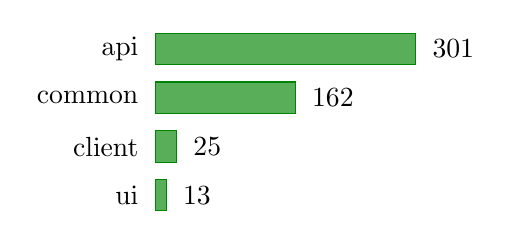
\begin{tikzpicture}[x=0.011cm, y=0.62cm, every node/.style={font=\normalsize}]
        \foreach \i/\n/\l in {1/301/{api}, 2/162/{common}, 3/25/{client}, 4/13/{ui}}{
          \node[anchor=east] at (-8,-\i) {\l};
          \draw[accent, fill=accent!65] (0,-\i-0.32) rectangle (\n,-\i+0.32);
          \node[anchor=west] at (\n+8,-\i) {\n};
        }
      \end{tikzpicture}

      {\small api: máy chủ; common: mã dùng chung; client: máy khách; ui: thành phần giao diện. Tổng 501 của cả kho, trong đó ít nhất 44 bài của sinh viên. Một bài bỏ qua có chủ đích, có sẵn từ Ghostfolio.}
    \end{column}
    \begin{column}{0.48\textwidth}
      \begin{itemize}
        \item TDD: viết bài kiểm tra trước, mã sau
        \item Kiểm thử độc lập bằng tác tử AI (Claude): 35 lỗi, đã sửa 10 lỗi Major
        \item Chưa chạy: đợt hai và Cypress (kiểm thử tự động trên trình duyệt)
      \end{itemize}
    \end{column}
  \end{columns}

\end{frame}
\note{1 phút. Nói rõ người kiểm thử độc lập là một tác tử AI, không phải người. 501 là cả kho, ít nhất 44 bài là của sinh viên.}

% 35 ------------------------------------------------------------
\begin{frame}[t]{Hạn chế đã biết và hướng khắc phục}
  \centering
  \begin{tabular}{@{}L{6.4cm}L{6.2cm}@{}}
    \toprule
    \textbf{Hạn chế} & \textbf{Hướng khắc phục} \\
    \midrule
    Lợi suất kỳ vọng từ lịch sử nhiễu & Dùng Black-Litterman; thử ước lượng khác \\
    Hiệp phương sai nhiễu khi ít dữ liệu & Co rút Ledoit và Wolf \cite{ledoit} \\
    Cân bằng rủi ro chưa có trần & Thêm trần để so công bằng \\
    Kiểm tra ngược chưa tính phí, thuế; một cấu hình & Thêm phí, thuế; nhiều cấu hình \\
    Hệ số 252 làm thấp lợi suất khi có tiền mã hóa & Suy hệ số từ tần suất thực tế \\
    Thời gian chạy đo một lần, sáu tài sản & Đo lặp với 20 tài sản \\
    Chưa chạy Cypress và đợt kiểm thử hai; lỗi D20, D24 còn mở & Chạy trong tích hợp liên tục \\
    \bottomrule
  \end{tabular}

  \vspace{4pt}
  Khối Black-Litterman ở trang Phân bổ chưa nhận quan điểm. Dữ liệu demo mô phỏng nên kết quả chỉ minh họa cách dùng.
\end{frame}
\note{1 phút. Đọc nhanh cột trái, nhấn ba mục: cân bằng rủi ro chưa trần, kiểm tra ngược chưa tính phí thuế, thời gian chạy mới đo một lần.}

% 36 ------------------------------------------------------------
\begin{frame}[t]{Kết luận}
  \centering\small
  \begin{tabular}{@{}L{2.2cm}L{10.6cm}@{}}
    \toprule
    \textbf{Mục} & \textbf{Kết quả} \\
    \midrule
    CH1 & Có: Việt hóa Ghostfolio, tiền mặc định VND, không viết lại hệ thống \\
    CH2, H1 & Có, trong phạm vi đã đo: 3 phương pháp, 6 tài sản, 1,7 đến 3,5 giây; 20 tài sản chưa đo \\
    CH3, H2, H3 & Có: kiểm thử theo tính chất; tỷ trọng hợp lệ, quan điểm tăng giá làm tăng tỷ trọng \\
    Ngoài mẫu & \textbf{Sharpe tối đa lỗ 4,5\%}, chia đều lãi 2,9\%, hiện tại lãi 1,8\%: chưa vượt chiến lược 1/N \\
    \bottomrule
  \end{tabular}

  \vspace{6pt}
  \begin{block}{Khuyến nghị}
    \small Không dùng hệ thống để ra quyết định đầu tư thật khi chưa kiểm chứng trên dữ liệu thị trường thật.
  \end{block}
  \vspace{-2pt}
  {\small Hai bài học: viết kiểm thử trước để giữ thuật toán đúng; kiểm thử độc lập tìm lỗi người viết mã không thấy.}
\end{frame}
\note{1,5 phút. Trả lời từng câu hỏi và giả thuyết. Nhấn khuyến nghị: không dùng để đầu tư thật khi chưa kiểm chứng trên dữ liệu thật.}

% 37 ------------------------------------------------------------
\begin{frame}[t]{Công trình khoa học: 12 bản thảo, 2 bài đã xuất bản}
  \begin{columns}[T]
    \begin{column}{0.40\textwidth}
      \centering
      \begin{tikzpicture}[x=0.5cm, y=0.62cm, every node/.style={font=\footnotesize}]
        \foreach \i/\n/\l/\c in {1/2/{Đã xuất bản}/accent, 2/1/{Đã duyệt đăng}/neutral, 3/1/{Sửa xong vòng 2}/neutral, 4/1/{Chờ duyệt đăng}/neutral, 5/3/{Đang sửa, phản biện}/neutral, 6/4/{Ở biên tập viên}/neutral}{
          \node[anchor=east] at (-0.15,-\i) {\l};
          \draw[\c, fill=\c!60] (0,-\i-0.3) rectangle (\n,-\i+0.3);
          \node[anchor=west] at (\n+0.12,-\i) {\n};
        }
      \end{tikzpicture}

      {\small Số bài theo giai đoạn (tổng 12)}
    \end{column}
    \begin{column}{0.58\textwidth}
      \footnotesize\setlength{\tabcolsep}{3pt}\renewcommand{\arraystretch}{1.05}
      \begin{tabular}{@{}rL{4.4cm}L{2.0cm}@{}}
        \toprule
        & \textbf{Tên bài} & \textbf{Tình trạng} \\
        \midrule
        1 & Black-Litterman optimization with regime switching CAPM and ABC-MCMC: Vietnamese stock market 2019-2025 & Đã xuất bản \\
        2 & Tiền gửi không kỳ hạn và ổn định tài chính ngân hàng: mô hình ngưỡng tại Việt Nam & Đã xuất bản \\
        3 & GRI adoption and corporate brownwashing: ASEAN-5 & Đã duyệt đăng \\
        4 & Inverse Black-Litterman and clustering machine learning: Vietnamese bank stocks & Sửa xong vòng 2 \\
        \bottomrule
      \end{tabular}
    \end{column}
  \end{columns}

  \vspace{2pt}
  {\small Bốn bài nổi bật; tám bài còn lại và tên đầy đủ ở slide dự phòng.}
\end{frame}
\note{1 phút. Chỉ hai bài đầu là công bố chính thức; các bài còn lại có thể thay đổi sau phản biện. Bài 1 và 4 gần đề tài nhất.}

% 38 ------------------------------------------------------------
\begin{frame}[t]{Tài liệu tham khảo}
  \fontsize{8}{9.6}\selectfont\vspace{-6pt}
  \begin{columns}[T]
    \begin{column}{0.49\textwidth}
      \begin{thebibliography}{99}
      \bibitem{markowitz} H. Markowitz, ``Portfolio selection,'' \emph{The Journal of Finance}, vol.~7, no.~1, pp.~77--91, 1952.
      \bibitem{agpl} Free Software Foundation, \emph{GNU Affero General Public License, version 3}, 2007.
      \bibitem{sharpe} W. F. Sharpe, ``Mutual fund performance,'' \emph{The Journal of Business}, vol.~39, no.~1, pp.~119--138, 1966.
      \bibitem{rockafellar} R. T. Rockafellar and S. Uryasev, ``Optimization of conditional value-at-risk,'' \emph{The Journal of Risk}, vol.~2, no.~3, pp.~21--41, 2000.
      \bibitem{maillard} S. Maillard, T. Roncalli, and J. Teïletche, ``The properties of equally weighted risk contribution portfolios,'' \emph{The Journal of Portfolio Management}, vol.~36, no.~4, pp.~60--70, 2010.
      \bibitem{blitterman} F. Black and R. Litterman, ``Global portfolio optimization,'' \emph{Financial Analysts Journal}, vol.~48, no.~5, pp.~28--43, 1992.
      \end{thebibliography}
    \end{column}
    \begin{column}{0.49\textwidth}
      \begin{thebibliography}{99}
      \setcounter{enumiv}{6}
      \bibitem{heLitterman} G. He and R. Litterman, ``The intuition behind Black-Litterman model portfolios,'' Goldman Sachs Investment Management Research, working paper, 1999.
      \bibitem{ownpaper} T. V. Nguyen \emph{et al.}, ``Black-Litterman portfolio optimization using regime switching CAPM and ABC-MCMC,'' \emph{Journal of Policy and Development Research}, vol.~01, pp.~81--99, 2026.
      \bibitem{idzorek} T. M. Idzorek, ``A step-by-step guide to the Black-Litterman model,'' in \emph{Forecasting Expected Returns in the Financial Markets}, Elsevier, 2007, pp.~17--38.
      \bibitem{demiguel} V. DeMiguel, L. Garlappi, and R. Uppal, ``Optimal versus naive diversification: How inefficient is the 1/N portfolio strategy?'' \emph{The Review of Financial Studies}, vol.~22, no.~5, pp.~1915--1953, 2009.
      \bibitem{ledoit} O. Ledoit and M. Wolf, ``A well-conditioned estimator for large-dimensional covariance matrices,'' \emph{Journal of Multivariate Analysis}, vol.~88, no.~2, pp.~365--411, 2004.
      \end{thebibliography}
    \end{column}
  \end{columns}
\end{frame}
\note{Slide tham khảo, không tính thời gian.}

% 39 ------------------------------------------------------------
\begin{frame}[t]{Cảm ơn và xin ý kiến}
  \centering
  
\includegraphics[height=1.6cm]{img/goc/ptit-logo.jpeg}

  \Large Xin cảm ơn thầy cô và anh chị đã lắng nghe

  \vspace{8pt}\normalsize
  \begin{tabular}{@{}rl@{}}
    Mã nguồn: & \url{https://github.com/trungcandygit/TTTN_Nguyen_Van_Trung} \\
    Giấy phép: & AGPL-3.0; dữ liệu demo là mô phỏng \\
    Liên hệ: & 15233582@st.neu.edu.vn \\
  \end{tabular}
\end{frame}
\note{0,5 phút. Cảm ơn và mời đặt câu hỏi. Mở slide dự phòng theo câu hỏi.}

% ======================= Slide dự phòng (không tính thời gian) =======================
\appendix

\begin{frame}{Dự phòng 1: sơ đồ tổ chức của ITMV}
  \centering
  \fig[0.68]{img/so-do-to-chuc.png}

  {\small Sinh viên vẽ lại theo tài liệu chưa công bố; chưa phải văn bản chính thức của công ty.}
\end{frame}
\note{Chỉ mở khi được hỏi về đơn vị thực tập.}


\begin{frame}{Dự phòng 2: các thực thể dữ liệu của dự án}
  \centering
  \fig[0.68]{img/du-lieu.png}

\end{frame}
\note{Chỉ mở khi được hỏi về cấu trúc dữ liệu.}


\begin{frame}{Dự phòng 3: thống kê và tỷ trọng của tám tài sản}
  \centering\scriptsize\setlength{\tabcolsep}{3pt}
  \begin{tabular}{@{}lrrrrrrr@{}}
    \toprule
    Tài sản & Lợi suất & Biến động & Hiện tại & Chia đều & Nghịch đảo biến động & Cân bằng rủi ro & Sharpe tối đa \\
    \midrule
    NVIDIA & 29,7\% & 56,2\% & 22,0\% & 12,5\% & 3,0\% & 2,7\% & 7,7\% \\
    Vietcombank & 10,2\% & 27,3\% & 13,8\% & 12,5\% & 6,3\% & 4,8\% & 6,8\% \\
    Quỹ trái phiếu VFMVFB & 9,5\% & 2,9\% & 13,4\% & 12,5\% & 58,1\% & 65,1\% & 40,0\% \\
    Vanguard S\&P 500 ETF & 8,6\% & 17,0\% & 12,1\% & 12,5\% & 10,1\% & 8,2\% & 27,0\% \\
    Vinamilk & 9,9\% & 26,8\% & 11,3\% & 12,5\% & 6,4\% & 5,0\% & 8,2\% \\
    FPT Corp & 12,1\% & 32,5\% & 10,4\% & 12,5\% & 5,3\% & 4,5\% & 10,3\% \\
    Hòa Phát & −4,1\% & 40,1\% & 8,8\% & 12,5\% & 4,3\% & 3,6\% & 0,0\% \\
    Microsoft & −3,8\% & 25,9\% & 8,4\% & 12,5\% & 6,6\% & 6,2\% & 0,0\% \\
    \bottomrule
  \end{tabular}

  \vspace{4pt}
\end{frame}
\note{Chỉ mở khi được hỏi về số liệu chi tiết của tám tài sản.}


\begin{frame}{Dự phòng 4: công trình khoa học, bản thảo 1 đến 6}
  \centering\scriptsize\renewcommand{\arraystretch}{1.05}
  \begin{tabular}{@{}rL{6.5cm}L{3.7cm}L{2.0cm}@{}}
    \toprule
    & \textbf{Tên bài} & \textbf{Nơi đăng} & \textbf{Tình trạng} \\
    \midrule
    1 & Black-Litterman portfolio optimization using regime switching CAPM and ABC-MCMC: Empirical evidence from the Vietnamese stock market period 2019-2025 & Journal of Policy and Development Research; trong nước & Đã xuất bản \\
    2 & Tiền gửi không kỳ hạn, hiệu quả hoạt động và ổn định tài chính ngân hàng: Bằng chứng từ mô hình ngưỡng tại Việt Nam & Tạp chí Kinh tế - Luật và Ngân hàng; trong nước & Đã xuất bản \\
    3 & GRI adoption and corporate brownwashing: Board governance evidence from ASEAN-5 & Int. J. of Management and Sustainability; Scopus Q3 & Đã duyệt đăng \\
    4 & Portfolio optimization with the inverse Black-Litterman framework and clustering machine-learning models: Evidence from Vietnamese bank stocks & Multidisciplinary Science Journal; Scopus Q3 & Đã sửa xong vòng 2 \\
    5 & Tác động của cấu trúc sở hữu lên ổn định tài chính của các ngân hàng thương mại Việt Nam & Tạp chí Kinh tế - Luật và Ngân hàng; trong nước & Chờ duyệt đăng sau 2 vòng \\
    6 & Limits to arbitrage in the Vietnamese physical gold market: The failure of short-term momentum & Journal of Economic and Banking Studies; trong nước & Đang sửa vòng 1 \\
    \bottomrule
  \end{tabular}
\end{frame}
\note{Các bản thảo 1 đến 6.}


\begin{frame}{Dự phòng 5: công trình khoa học, bản thảo 7 đến 12}
  \centering\scriptsize\renewcommand{\arraystretch}{1.05}
  \begin{tabular}{@{}rL{6.5cm}L{3.7cm}L{2.0cm}@{}}
    \toprule
    & \textbf{Tên bài} & \textbf{Nơi đăng} & \textbf{Tình trạng} \\
    \midrule
    7 & Corporate brownwashing and firm valuation in ASEAN-5 disclosure regimes & Cogent Business \& Management; ESCI, Scopus Q2 & Đang phản biện vòng 1 \\
    8 & Structural breaks in Vietnamese stock market liquidity: Evidence from the Amihud illiquidity measure and Bai-Perron regime-shift detection & Asian Journal of Economics and Banking & Đang tìm phản biện \\
    9 & Nested equity index correlations overstate true co-movement: Evidence from Vietnam & Asia-Pacific Financial Markets; Scopus Q2 & Ở biên tập viên \\
    10 & Who gains from a market upgrade? Stock liquidity and prices around Vietnam's FTSE Russell reclassification & Finance Research Open; Elsevier & Ở biên tập viên \\
    11 & Rated at the peak? Firm valuation around the first LSEG ESG score in five Southeast Asian markets & Sustainable Finance Review; Emerald Publishing & Ở biên tập viên \\
    12 & Sales-based real earnings management and the cost of debt: Evidence from five ASEAN markets & Accounting Open; Elsevier & Ở biên tập viên \\
    \bottomrule
  \end{tabular}

  \vspace{2pt}
  {\scriptsize Sinh viên là tác giả liên hệ của cả 12 bài; chỉ hai bài đầu là công bố chính thức.}
\end{frame}
\note{Các bản thảo 7 đến 12.}




\end{document}
